\section{程序混淆类}
\begin{center}
    只要代码足够乱, 就没人发现我写错.  \\
                \hfill --- 网上 $\cdot$ 佚名
\end{center}

\subsection{背景知识}
程序混淆(program obfuscation)是一种编译的方法技术, 它将容易理解的源程序转化成难以理解的形式, 同时保持原有功能性不变. 
程序混淆概念起源于上世界70年代的代码混淆领域, 在软件保护领域(如软件水印、防逆向工程)有着广泛的应用, 然而一直缺乏严格的安全定义. 

\begin{figure}[!hbtp]
\begin{center}
\begin{tikzpicture}
    \node [name=C, textnode] {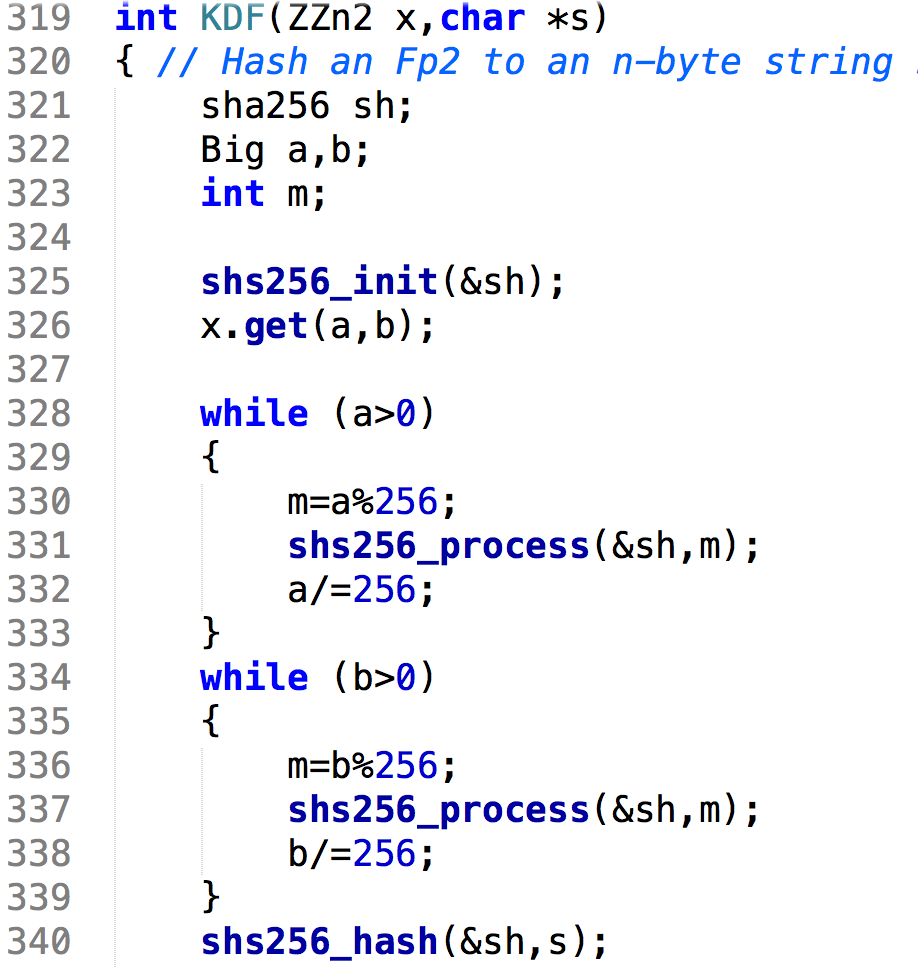
\includegraphics[width=1.2in]{figure/code.png}};
    \node [name=OC, textnode, right of=C, xshift=16em] {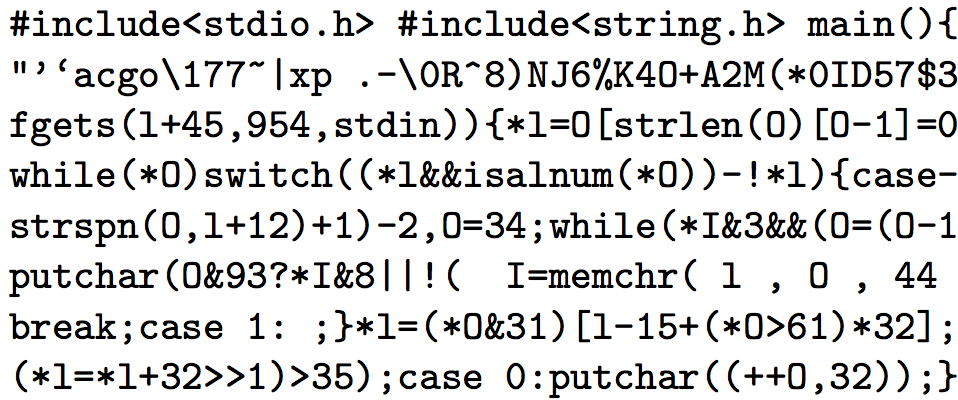
\includegraphics[width=1.2in]{figure/obf.png}};
    \draw (C) edge[->] node[above] {$\mathcal{O}$} (OC);
\end{tikzpicture}
\end{center}
\caption{程序混淆}
\end{figure}

Barak等~\cite{Barak-CRYPTO-2001}首次将程序混淆引入密码学领域, 将程序从狭义的代码泛化为广义的算法, 
同时提出了虚拟黑盒(VBB, virtual black-box)混淆的严格定义. 

\begin{figure}[!hbtp]
\begin{center}
\begin{tikzpicture}
    \node [rectanglenode, name=C, minimum width=6em, minimum height=3em] {$C$};
    \node [name=OC, rectanglenode, fill=gray, right of=C, xshift=12em, minimum width=6em, minimum height=3em] {~$\mathcal{O}(C)$~};
    \node [name=BC, rectanglenode,  fill=black, below of=OC, yshift=-6em, minimum width=6em, minimum height=3em] {};
    \draw (C) edge[->] node[above] {$\mathcal{O}$} (OC);
    \node [textnode, below of=OC, yshift=-3em] {$\approx_c$};
\end{tikzpicture}
\end{center}
\caption{虚拟黑盒混淆}
\end{figure}

我们回顾不可区分混淆(indistinguishability obfuscator, $\iO$)~\cite{Garg-FOCS-2013}如下. 
\begin{definition}[虚拟黑盒混淆]
我们称一个uniform PPT machine $\iO$是电路簇$\{\mathcal{C}_\kappa\}$的不可区分混淆器当且仅当其满足以下两个条件:
\begin{itemize}
\item 功能保持: 对于任意安全参数$\kappa \in \mathbb{N}$、任意的$C \in \mathcal{C}_\kappa$和所有输入$x \in \{0,1\}^*$有:
    \begin{equation*}
        \Pr[C'(x) = C(x): C' \leftarrow \iO(\kappa, C)] = 1
    \end{equation*} 

\item 虚拟黑盒混淆: 存在PPT的模拟器$\mathcal{S}$, 对于任意$C \in \{\mathcal{C}_\kappa\}$, 对于任意PPT敌手$\mathcal{A}$, 
	我们有: 
    \begin{equation*}
        \mathcal{A}(\mathcal{O}(C)) \approx_c \mathcal{S}^{C}
    \end{equation*}   
    其中公式左边表示$\mathcal{A}$的视图, 公式右边表示$\mathcal{S}$在通过对$C$进行黑盒访问所输出的视图. 
\end{itemize} 
\end{definition}

\begin{note}
虚拟黑盒混淆的定义是基于模拟的游戏, 刻画的是PPT敌手从混淆程序$\mathcal{O}(C)$中获取的任何信息不会比黑盒访问$C$获得的信息更多. 
换言之, 掌握$\mathcal{O}(C)$的敌手视图可以由模拟器通过黑盒访问$C$模拟得出. 
VBB试图隐藏程序$C$的所有细节. 比如$C$以平方差公式计算$x^2-1$, 即$C(x) = (x+1)(x-1)$. 
那么敌手在获得$\mathcal{O}(C)$后, 掌握的所有信息等价输入/输出元组$(x, x^2-1)$, i.e., $(1, 0)$, $(2, 3)$, $(3, 8)$, $\dots$
\end{note}

VBB的混淆定义强到极致, 因此在密码学中应用起来颇为简单直观. 
事实上, 在1976年Diffie和Hellman的划时代论文~\cite{DH-IEEE-IT-1976}中, 
就已经提出了利用混淆器将对称加密方案编译为公钥加密方案的想法(如图~\ref{figure:Diffie-Hellman-idea}): 
\begin{enumerate}
    \item 将对SKE的加密算法$\mathsf{Enc}(sk, m, r)$中的第一个输入hardwired进电路, 得到$\mathsf{Enc}_{sk}(m, r)$; 
    \item 利用混淆器编译$\mathsf{Enc}_{sk}(\cdot, \cdot)$, 将得到的混淆程序作为公钥$pk$.
\end{enumerate}

\begin{figure}[!hbtp]
\begin{center}
\begin{tikzpicture}
    \node [rectanglenode, name=enc, minimum width=5em, minimum height=2em] {$\mathsf{Enc}$};
    \node [textnode, name=sk, above of=enc, xshift=-3em, yshift=3em, color=red] {$sk$}; 
    \node [textnode, name=m, above of=enc, xshift=0em, yshift=3em] {$m$}; 
    \node [textnode, name=r, above of=enc, xshift=3em, yshift=3em] {$r$};
    \node [textnode, name=c, below of=enc, yshift=-3em] {$c$}; 
    \draw (sk) edge[->] (enc);
    \draw (m) edge[->]  (enc);
    \draw (r) edge[->]  (enc);
    \draw (enc) edge[->] (c);

    \node [rectanglenode, name=dec, right of=enc, xshift=16em, minimum width=5em, minimum height=2em] {$\mathsf{Dec}$};
    \node [textnode, name=sk1, above of=dec, xshift=-3em, yshift=3em, color=red] {$sk$}; 
    \node [textnode, name=c1, above of=dec, xshift=3em, yshift=3em] {$c$}; 
    \node [textnode, name=m1, below of=dec, yshift=-3em] {$m$}; 
    \draw (sk1) edge[->] (dec);
    \draw (c1) edge[->]  (dec);
    \draw (dec) edge[->] (m1);

    \node [rectanglenode, name=enc2, below of=enc, yshift=-12em, minimum width=5em, minimum height=2em] {$\mathsf{Enc}_{\red{sk}}$}; 
    \node [textnode, name=m2, above of=enc2, xshift=-3em, yshift=3em] {$m$}; 
    \node [textnode, name=r2, above of=enc2, xshift=3em, yshift=3em] {$r$};
    \node [textnode, name=c2, below of=enc2, yshift=-3em] {$c$}; 
    \draw (m2) edge[connect]  (enc2);
    \draw (r2) edge[connect]  (enc2);
    \draw (enc2) edge[connect] (c2);

    \draw (sk) edge[->, bend left=-45] node[right] {hardwired} (enc2.west);

    \node [rectanglenode, fill = gray, name=enc3, right of=enc2, xshift=16em, minimum width=5em, minimum height=2em] 
        {$\mathcal{O}(\mathsf{Enc}_{sk})$}; 
    \node [textnode, name=m3, above of=enc3, xshift=-3em, yshift=3em] {$m$}; 
    \node [textnode, name=r3, above of=enc3, xshift=3em, yshift=3em] {$r$};
    \node [textnode, name=c3, below of=enc3, yshift=-3em] {$c$}; 
    \draw (m3) edge[->]  (enc3);
    \draw (r3) edge[->]  (enc3);
    \draw (enc3) edge[->] (c3);

    \node [textnode, name=pk, right of=enc3, xshift=5em] {$pk$}; 
    \draw (enc3) edge[->] (pk);

    \draw (enc2) edge[->] node[above] {obfuscate} (enc3);
\end{tikzpicture}
\end{center}
\caption{SKE $\Rightarrow$ PKE via obfuscation}\label{figure:Diffie-Hellman-idea}
\end{figure}

VBB的安全定义至强, Barak等~\cite{Barak-CRYPTO-2001}指出VBB``too good to be true!''--不存在针对任意电路(通用, general-purpose)的VBB. 
VBB因为安全太强以至于不存在, Garg等~\cite{Garg-FOCS-2013}降低了安全性要求, 引入了不可区分混淆(indistinguishability obfuscator, $\iO$). 
\begin{definition}[不可区分混淆($\iO$)]
我们称一个uniform PPT machine $\iO$是电路簇$\{\mathcal{C}_\kappa\}$的不可区分混淆器当且仅当其满足以下两个条件:
\begin{itemize}
\item 功能保持: 对于任意安全参数$\kappa \in \mathbb{N}$、任意的$C \in \mathcal{C}_\kappa$和所有输入$x \in \{0,1\}^*$有:
    \begin{equation*}
        \Pr[C'(x) = C(x): C' \leftarrow \iO(\kappa, C)] = 1
    \end{equation*} 

\item 不可区分混淆: 对于任意PPT敌手$(\mathcal{S}, \mathcal{D})$, 存在关于安全参数的可忽略函数$\alpha$使得: 
    如果$\Pr[\forall x, C_0(x) = C_1(x): (C_0, C_1, aux) \leftarrow \mathcal{S}(\kappa)] \geq 1 - \alpha(\kappa)$, 
    那么我们有: 
    \begin{equation*}
        \left|\Pr[\mathcal{D}(aux, \iO(\kappa, C_0)) = 1] - 
        \Pr[\mathcal{D}(aux, \iO(\lambda, C_1)) = 1]\right| \leq \alpha(\kappa)
    \end{equation*}   
\end{itemize} 
\end{definition}

\begin{figure}[!hbtp]
\begin{center}
\begin{tikzpicture}
    \node [rectanglenode, name=C0, minimum width=6em, minimum height=3em] {$C_0$};
    \node [name=C1, rectanglenode, below of=C0, minimum width=6em, minimum height=3em, yshift=-8em] {$C_1$};
    \node [name=OC0, rectanglenode,  fill=gray, right of=C0, xshift=12em, minimum width=6em, minimum height=3em] {$\iO(C_0)$};
    \node [name=OC1, rectanglenode, fill=gray, right of=C1, xshift=12em, minimum width=6em, minimum height=3em] {$\iO(C_1)$};
    \draw (C0) edge[->] node[above] {$\iO$} (OC0);
    \draw (C1) edge[->] node[above] {$\iO$} (OC1);
    \node [textnode, below of=C0, yshift=-4em] {$\equiv$};
    \node [textnode, below of=OC0, yshift=-4em] {$\approx_c$};
\end{tikzpicture}
\end{center}
\caption{不可区分混淆示意图}
\end{figure}


\begin{remark}
\begin{itemize}
\item 不可区分混淆的定义类似加密方案的不可区分性, 对于任意功能相同的电路$C_0$和$C_1$, 均有$\iO(C_0) \approx_c \iO(C_1)$. 
    这里, 我们可以把电路$C$类比为消息, $\iO$类比为加密算法. 与VBB试图隐藏电路的所有信息不同, 
    $\iO$只试图隐藏电路的部分信息: 比如$C_0(x) = (x+1)(x-1)$, $C_1(x) = (x+2)(x-2)+3$,    
    那么如果混淆后的程序均是$x^2-1$即可满足不可区分安全性.
    非严格的说, $\iO$试图在以统一的方式完成同质的计算. 

\item 在上述定义中, 条件\redul{$\Pr[\forall x, C_0(x) = C_1(x): (C_0, C_1, aux) \leftarrow \mathcal{S}(\kappa)] \geq 1 - \alpha(\kappa)$}
    并不意味着$C_0$和$C_1$存在差异输入(differing-inputs), 而指的是$C_0$和$C_1$以极高的概率功能性完全相同, 
    这一点体现在概率空间定义在$\mathcal{S}$的随机带而与$x$无关. 

\item $aux$表示$\mathcal{S}$在采样$C_0, C_1$过程中得到的任意信息, 用于辅助$\mathcal{D}$区分$\iO(C_0)$和$\iO(C_1)$. 
\end{itemize}
\end{remark}

\begin{trivlist}
\item \textbf{差异输入混淆.} 如果在上述$\iO$定义中, 将$\mathcal{S}$所采样两个电路的要求由功能性完全相同放宽为允许存在差异输入, 
    则得到的是更强的混淆器, 称为差异输入混淆($\diO$, differing-input obfuscation). 
    \cite{BCP-TCC-2014}中给出了正面结果: 证明了$\iO$蕴含多项式级别差异输入规模的$\diO$. 
    \cite{BSW-EUROCRYPT-2016}中给出了负面结果: 证明了亚指数安全(sub-exponentially secure)的单向函数存在, 
    则针对无界输入Turing machine(TMs with unbounded inputs)亚指数安全的$\diO$不存在.  
\end{trivlist}

我们再把注意力转回不可区分混淆. 如上所述, VBB易用但对于通用电路并不存在, $\iO$弱化了安全要求, 从而有了基于合理困难性假设的构造. 
安全性弱化后$\iO$是否还有着强大的威力? 如何去应用呢? 
直观上: 混淆后的程序既可以保持功能性, 又能够在某种程度上隐藏常量. 
常量皆程序. 在密码学中, 公钥和私钥均可以看做一段程序, 其中硬编码(hardwired)原本的公钥和私钥作为常量: 比如加密就是以明文和随机数为输入, 运行``公钥程序'', 输出密文; 
解密就是以密文为输入, 运行``解密程序'', 输出明文. 
混淆在密码学中的一类强大应用就是完成从Minicrypt到Cryptomania的穿越, 因为借助混淆, 可以在不泄漏秘密的情况下以公开的方式执行某个任务.  
\begin{itemize}
    \item 保持功能性 $\Rightarrow$ 确保密码方案的功能性
    \item 在某种程度上隐藏常量(对应需要保护的秘密) $\Rightarrow$ 确保密码方案的安全性
\end{itemize}

\begin{remark}
混淆的威力强大如魔法, 其力量的来源在于对底层密码组件的调用方式是非黑盒的(non-black-box), 因此可以绕过黑盒意义下的不可能结果(black-box impossibilities). 
\end{remark}

在$\iO$提出后最初的一段时间, 应用只局限于属性加密(ABE). 
原因是应用$\iO$设计密码方案并非易事, 需要解决的技术难题是精准的隐藏``部分信息''. 
2014年, Sahai和Waters~\cite{SW-STOC-2014}创造性的发展了可穿孔编程技术(puncture program technique), 
以此给出了应用$\iO$的范式, 展示了$\iO$的巨大威力--结合单向函数和$\iO$重构了几乎所有的密码组件, 
包括公钥加密/密钥封装、可否认加密、数字签名、单向陷门函数、非交互式零知识证明、不经意传输等.

\subsection{受限伪随机函数}
以下首先介绍可穿孔编程技术的关键密码组件---受限伪随机函数(constrained PRF). 
对于标准的伪随机函数$F: K \times X \rightarrow Y$, 密钥$k$不支持代理, 因此求值方式是``完全或无''(all-or-nothing):
\begin{itemize}
    \item 知晓密钥$k$时, 可以对定义域中的所有点$x \in X$进行函数求值, 得到$F_k(x)$.
    \item 不知晓密钥$k$时, $F_k(\cdot)$是伪随机的. 
\end{itemize}

三组科学家~\cite{BW-ASIACRYPT-2013, KPTZ-CCS-2013, BGI-PKC-2014}独立并行的提出了受限伪随机函数(constrained PRF). 
在受限伪随机函数中, $k$可以进一步代理得到受限密钥, 受限密钥可以对定义域中的部分输入进行求值. 正式的定义如下: 
\begin{definition}[受限伪随机函数(constrained PRF)] 
受限伪随机函数包含以下多项式时间算法: 
\begin{itemize}
\item $\mathsf{Setup}(1^\kappa)$: 以安全参数为输入, 输出公开参数$pp$, 其中包含了函数$F: K \times X \rightarrow Y$的描述
    以及电路族$\mathcal{C} = \{f: X \rightarrow \{0,1\}\}$的描述. 

\item $\mathsf{KeyGen}(pp)$: 随机采样密钥$k \sample K$. 

\item $\mathsf{Constrain}(k, f)$: 以密钥$k$和$c \in \mathcal{C}$为输入, 输出受限密钥$k_f$. 

\item $\mathsf{Eval}(k/k_f, x) = F_k(x)$: 以密钥$k$或受限密钥$k_c$和$x \in X$为输入, 当第一输入为$k$时输出$F_k$, 
    当第一输入为$k_c$时, 如果$f(x)=1$则输出$F_k(x)$, 否则输出$\bot$. 
\end{itemize}
\end{definition}

\begin{trivlist}
\item \textbf{安全性.} 受限伪随机函数要求对于没有被受限密钥和求值询问覆盖的输入, 其输出仍然是伪随机的. 
    定义敌手$\mathcal{A} = (\mathcal{A})$的优势函数如下: 
\begin{displaymath}
    \Pr \left[\beta = \beta': 
    \begin{array}{l}
        pp \leftarrow \mathsf{Setup}(1^\lambda); \\
        k \leftarrow \mathsf{KeyGen}(pp); \\
        (x^*, state) \leftarrow \mathcal{A}_1^{\Oeval, \Oconstrain}(pp);\\
        \beta \sample \{0, 1\}, y_0^* = F_k(x^*), y_1^* \sample Y; \\
        \beta' \leftarrow \mathcal{A}_2^{\Oeval, \Oconstrain}(state, y_\beta^*);
    \end{array}
    \right] - \frac{1}{2}.
\end{displaymath}
其中$\Oeval$表示求值谕言机, 以$x \in X$为输入, 返回$F_k(x)$; 
$\Oconstrain$表示受限密钥谕言机, 以$c \in \mathcal{C}$为输入, 输出$k_c$. 
在安全试验过程中, 挑战者隐式的维护集合$H$以记录被已发起的受限密钥询问和求值询问覆盖的定义域中元素.  
为了避免定义无意义, $\mathcal{A}_1$在第一阶段被禁止选择$H$中的元素作为挑战点, 
$\mathcal{A}_2$在第二阶段被禁止发起能够覆盖挑战点的受限密钥询问和求值询问. 
如果任意的PPT敌手$\mathcal{A}$在上述游戏中的优势函数均为可忽略函数, 则称受限伪随机函数是安全的. 
\end{trivlist}

\begin{remark}
对任意$\mathcal{C}$, 均存在平凡的受限伪随机函数构造: 受限密钥生成函数通过枚举的方式生成受限密钥, 即$k_f = \{y = F_k(x)\}_{f(x)=1}$. 
为了排除此类平凡的构造, 我们要求受限密钥是紧致的, 即对于$\forall f \in \mathcal{C}$, 均有$|k_f| = \kappa^{O(1)}$. 
\end{remark}

Sahai和Waters~\cite{SW-STOC-2014}引入了受限伪随机函数的特例——可穿孔伪随机函数(puncturable PRF), 正式定义如下: 
\begin{definition}[可穿孔伪随机函数(puncturable PRF)] 
可穿孔伪随机函数包含以下多项式时间算法: 
\begin{itemize}
\item $\mathsf{Setup}(1^\kappa)$: 以安全参数为输入, 输出公开参数$pp$, 其中包含了函数$F: K \times X \rightarrow Y$的描述
    和电路族$\mathcal{C} = \{f_{x^*}: X \rightarrow \{0,1\}\}_{x^* \in X}$的描述.  
    $f_{x^*}(\cdot)$的具体定义是$f_{x^*}(x) = \neg x^* \stackrel{?}{=}x$. 为了表述简洁, 以下在不引起混淆的情况下使用$x^*$表征$f_{x^*}$.   

\item $\mathsf{KeyGen}(pp)$: 随机采样密钥$k \sample K$. 

\item $\mathsf{Puncture}(k, x^*)$: 以密钥$k$和$x^* \in X$为输入, 输出受限密钥$k_{x^*}$. 

\item $\mathsf{Eval}(k/k_{x^*}, x)$: 以密钥$k$或受限密钥$k_{x^*}$和$x \in X$为输入, 当第一输入为$k$时输出$F_k$, 
    当第一输入为$k_{x^*}$时, 如果$x \neq x^*$时输出$F_k(x)$, 否则输出$\bot$. 
\end{itemize}
\end{definition}

可穿孔伪随机函数的安全定义直觉是对于没有被受限密钥覆盖的输入, 其输出仍然是伪随机的. 存在以下两种等价定义. 
\begin{trivlist}
\item \textbf{选择伪随机性.} 定义敌手$\mathcal{A} = (\mathcal{A}_1, \mathcal{A}_2)$的优势函数如下: 
\begin{displaymath}
    \Pr \left[\beta = \beta': 
    \begin{array}{l}
        (x^*, state) \leftarrow \mathcal{A}_1(\kappa);\\
        pp \leftarrow \mathsf{Setup}(1^\lambda); \\
        k \leftarrow \mathsf{KeyGen}(pp); \\
        k_{x^*} \leftarrow \mathsf{Puncture}(k, x^*);\\ 
        \beta \sample \{0, 1\}, y_0^* = F_k(x^*), y_1^* \sample Y; \\
        \beta' \leftarrow \mathcal{A}_2(state, k_x^*, y_\beta^*);
    \end{array}
    \right] - \frac{1}{2}.
\end{displaymath}
如果任意的PPT敌手$\mathcal{A}$在上述游戏中的优势函数均为可忽略函数, 则称可穿孔伪随机函数是选择伪随机的. 
\end{trivlist}

\begin{figure}[!hbtp]
\begin{center}
\begin{tikzpicture}
    \node [name=adv, textnode] {
\includegraphics[width=0.5in]{figure/adversary.png}};
    \node [name=challenger, textnode, right of = adv, xshift=18em] 
        {
\includegraphics[width=0.5in]{figure/challenger.png}}; 

    \draw ($(adv.east)+(0em, 0.5em)$) edge[->] node[above] {$x^*$} ($(challenger.west)+(0em, 0.5em)$);

    \node [name=setup, textnode, right of=challenger, xshift = 9em, yshift = 1.5em] 
         {$pp \leftarrow \mathsf{Setup}(1^\kappa)$\\$k \sample K$, $\beta \sample \{0,1\}$\\$k_{x^*} \leftarrow \mathsf{Puncture}(k, x^*)$
         \\$y_0^* \leftarrow F(k, x^*)$; $y_1^* \sample Y$}; 
    \draw ($(challenger.west)+(0em, -1.5em)$) edge[->] node[above] {$pp$, $k_{x^*}$, $y_\beta^*$} ($(adv.east)+(0em, -1.5em)$);

    \draw ($(adv.east)+(0em, -3em)$) edge[->] node[above] {$\beta'$} ($(challenger.west)+(0em, -3em)$);
    \node [name=win, textnode, right of=challenger, xshift = 6.5em, yshift = -3em] {$\beta' = ? \beta$}; 
\end{tikzpicture}
\end{center}
\caption{可穿孔伪随机函数选择伪随机性示意图}
\end{figure}

\begin{trivlist}
\item \textbf{弱伪随机性.} 定义敌手$\mathcal{A} = (\mathcal{A}_1, \mathcal{A}_2)$的优势函数如下: 
\begin{displaymath}
    \Pr \left[\beta = \beta': 
    \begin{array}{l}
        pp \leftarrow \mathsf{Setup}(1^\lambda); \\
        k \leftarrow \mathsf{KeyGen}(pp), x^* \sample X; \\
        k_{x^*} \leftarrow \mathsf{Puncture}(k, x^*);\\ 
        \beta \sample \{0, 1\}, y_0^* = F_k(x^*), y_1^* \sample Y; \\
        \beta' \leftarrow \mathcal{A}(pp, x^*, k_x^*, y_\beta^*);
    \end{array}
    \right] - \frac{1}{2}.
\end{displaymath}
如果任意的PPT敌手$\mathcal{A}$在上述游戏中的优势函数均为可忽略函数, 则称可穿孔伪随机函数是弱伪随机的. 
\end{trivlist}

\begin{figure}[!hbtp]
\begin{center}
\begin{tikzpicture}
    \node [name=adv, textnode] {
\includegraphics[width=0.5in]{figure/adversary.png}};
    \node [name=challenger, textnode, right of = adv, xshift=18em] 
        {
\includegraphics[width=0.5in]{figure/challenger.png}}; 

    \draw ($(adv.east)+(0em, 0.5em)$) edge[<-] node[above] {$pp, x^*, k_{x^*}, y_\beta$} ($(challenger.west)+(0em, 0.5em)$);

    \node [name=setup, textnode, right of=challenger, xshift = 9em, yshift = 1.5em] 
         {$pp \leftarrow \mathsf{Setup}(1^\kappa)$\\$k \sample K$, $\beta \sample \{0,1\}$\\$x^* \sample X$, $k_{x^*} \leftarrow \mathsf{Puncture}(k, x^*)$
         \\$y_0^* \leftarrow F(k, x^*)$; $y_1^* \sample Y$}; 
    \draw ($(adv.east)+(0em, -1.5em)$)  edge[->] node[above] {$\beta'$} ($(challenger.west)+(0em, -1.5em)$);

    \node [name=win, textnode, right of=challenger, xshift = 6.5em, yshift = -3em] {$\beta' = ? \beta$}; 
\end{tikzpicture}
\end{center}
\caption{可穿孔伪随机函数弱伪随机性示意图}
\end{figure}
文献~\cite{Chen-ASIACRYPT-2018}证明了可穿孔弱伪随机函数的两种安全定义等价. 

\begin{remark}
在定义方面, 可穿孔伪随机函数中的受限密钥$k_{x^*}$求值功能是``全除一''的, 是ABO类型密钥. 
在安全性方面, 可穿孔伪随机函数要求弱伪随机性, 
即对于挑战者随机选择的点$x^*$, 即使拥有$k_x^*$, $F(x^*)$在敌手的视图中依然伪随机, 即: 
\begin{equation*}
     (pp, x^*, k_{x^*}, \red{F_k(x^*)}) \approx_c (pp, x^*, k_{x^*}, y^*), \text{其中~}y^* \sample Y
\end{equation*}

由于可穿孔伪随机函数的受限类型特殊, 因此安全定义相比一般的受限伪随机函数在形式上更加简单. 
\end{remark}

可穿孔伪随机函数可以通过GGM树形伪随机函数自然得出~\cite{BW-ASIACRYPT-2013, KPTZ-CCS-2013, BGI-PKC-2014}, 因此仍属于Minicrypt. 

\begin{figure}[!hbtp]
\begin{center}
\begin{tikzpicture}
% draw the root
\node [rectanglenode, dashed, name=root, minimum width=4em, minimum height=2em] {$s$};

% layer 1 
\node [rectanglenode, name=s0, dashed, below of=root, yshift=-5em, xshift=-8em, minimum width=4em, minimum height=2em] {$\mathsf{G}_0(s)$}; 
\node [rectanglenode, name=s1, below of=root, yshift=-5em, xshift=8em, minimum width=4em, minimum height=2em] {$\mathsf{G}_1(s)$}; 

% layer 2
\node [rectanglenode, name=s00, below of=s0, xshift=-5em, yshift=-5em, minimum width=4em, minimum height=2em] {$\mathsf{G}_0(\mathsf{G}_0(s))$}; 
\node [rectanglenode, name=s01, below of=s0, dashed, xshift=3.5em, yshift=-5em, minimum width=4em, minimum height=2em] {$\mathsf{G}_1(\mathsf{G}_0(s))$}; 

\node [rectanglenode, name=s10, below of=s1, xshift=-3.5em, yshift=-5em, minimum width=4em, minimum height=2em] {}; 
\node [rectanglenode, name=s11, below of=s1, xshift=5em, yshift=-5em,  minimum width=4em, minimum height=2em] {}; 

% leaf
\node [circlenode, name=l000, below of=s00, xshift=-2.2em, yshift=-5em, minimum width=2em] {}; 
\node [circlenode, name=l001, below of=s00, xshift=2.2em, yshift=-5em, minimum width=2em] {}; 

\node [circlenode, draw=blue!30, fill=blue!30, name=l010, below of=s01, xshift=-2.2em, yshift=-5em, minimum width=2em] {}; 
\node [textnode, name=l011, below of=s01, xshift=2.2em, yshift=-5em, minimum width=2em] {$\mathsf{G}_1(\mathsf{G}_1(\mathsf{G}_0(s)))$}; 

\node [circlenode, name=l100, below of=s10, xshift=-2.2em, yshift=-5em, minimum width=2em] {}; 
\node [circlenode, name=l101, below of=s10, xshift=2.2em, yshift=-5em, minimum width=2em] {}; 

\node [circlenode, name=l110, below of=s11, xshift=-2.2em, yshift=-5em, minimum width=2em] {}; 
\node [circlenode, name=l111, below of=s11, xshift=2.2em, yshift=-5em, minimum width=2em] {}; 


% arrows
\draw (root.south) edge[->, thick, red] node [above] {0} (s0.north);
\draw (root.south) edge[->, thin] (s1.north);

\draw (s0.south) edge[->, thin] (s00.north);
\draw (s0.south) edge[->, thick, red] node [above, xshift=0.4em, yshift=-0.5em] {1} (s01.north);
\draw (s1.south) edge[->, thin] (s10.north);
\draw (s1.south) edge[->, thin] (s11.north);

\draw ($(s00.south)$) edge[->, thin] (l000);
\draw ($(s00.south)$) edge[->, thin] (l001);
\draw ($(s01.south)$) edge[->, thick, red] node [above, xshift=-0.4em, yshift=-0.5em] {0} (l010);
\draw ($(s01.south)$) edge[->, thin] (l011);
\draw ($(s10.south)$) edge[->, thin] (l100);
\draw ($(s10.south)$) edge[->, thin] (l101);
\draw ($(s11.south)$) edge[->, thin] (l110);
\draw ($(s11.south)$) edge[->, thin] (l111);


\node [textnode, name=l0, right of = root, xshift=20em] {$0$}; 
\node [textnode, name=l1, below of = l0, yshift=-5em] {$1$}; 
\node [textnode, name=l2, below of = l1, yshift=-5em] {$2$}; 
\node [textnode, name=ln, below of = l2, yshift=-5em] {$3$}; 

\end{tikzpicture}
\end{center}
\caption{GGM construction: $k_{010} = \{\mathsf{G}_0(\mathsf{G}_0(s)), 
\mathsf{G}_1(\mathsf{G}_0(\mathsf{G}_0(s))), \mathsf{G}_1(s)\}$}
\end{figure}


\subsection{基于不可区分混淆的KEM构造}
本章将逐步的展示如何基于$\iO$构造KEM, 实现Diffie-Hellman当年的梦想. 

\begin{trivlist}
    \item \textbf{起点方案.} 首先将对称场景下基于PRF的KEM封装算法表达为程序的形式, 如下图所示.
\end{trivlist}

\begin{framed}
\vspace{-1em}
\begin{center}$\mathsf{Encaps}$\end{center}
\vspace{-1em}
\begin{trivlist}   
    \item Input: secret key {$\boxed{sk}$}, randomness $x$ 
        \begin{enumerate}\itemsep 1pt \parskip 0pt \parsep 0pt
            \item output $c = x$, $k \leftarrow \mathsf{PRF}(sk, c)$.
        \end{enumerate}
\end{trivlist}
\vspace{-1em}
\end{framed}
再对程序进行微调, 将$sk$由输入变为hardwired的常量, 如下图所示:  

\begin{framed}
\vspace{-1em}
\begin{center}$\mathsf{Encaps}$\end{center}
\begin{trivlist}
    \item \underline{Constants: secret key {$sk$}} 
    \item Input: randomness $x$ 
        \begin{enumerate}\itemsep 1pt \parskip 0pt \parsep 0pt
            \item output $c = x$, $k \leftarrow F(sk, c)$.
        \end{enumerate}
\end{trivlist}
\vspace{-1em}
\end{framed}

由于通用的VBB并不存在, 因此尝使用$\iO$对程序混淆, 将混淆后的结果作为公钥
\begin{equation*}
    pk \leftarrow \red{\iO}(\mathsf{Encaps})
\end{equation*}

\begin{trivlist}
\item \textbf{技术困难1.}在将KEM的IND-CCA安全性归约到PRF的伪随机性时, 会遇到以下矛盾点: 
\begin{itemize}
    \item 在构造层面, 归约算法$\mathcal{R}$需要掌握$sk$以生成$pk$  
    \item 为了让归约有意义, 归约算法$\mathcal{R}$不能掌握私钥$sk$ 
\end{itemize}  
\end{trivlist} 

观察到KEM的IND-CCA安全仅要求随机挑战密文$c^*$封装的会话密钥是伪随机的, 
因此消除矛盾点的核心想法是使用可穿孔伪随机函数替代标准伪随机函数, 在挑战密文$c^*$处穿孔:
\begin{itemize}
    \item 生成$sk_{c^*}$得以对$c^*$外的所有点求值, 同时保持$F_{sk}(c^*)$的伪随机性. 
    \item 利用$sk_{c^*}$替代$sk$构建程序并混淆生成公钥. 
\end{itemize}


\begin{framed}
\vspace{-1em}
\begin{center}$\mathsf{Encaps}$\end{center}

\begin{trivlist}
    \item Constants: secret key {$sk$}
    \item Input: randomness $x$ 
        \begin{enumerate}\itemsep 1pt \parskip 0pt \parsep 0pt
            \item output $c = x$, $k \leftarrow F(sk, c)$.
        \end{enumerate}
\end{trivlist}
\vspace{-1em}
\end{framed}
\begin{center}
    方案构造: $pk \leftarrow \iO(\mathsf{Encaps})$
\end{center}


\begin{framed}
\vspace{-1em}
\begin{center}$\mathsf{Encaps}^*$\end{center}
\begin{trivlist}
    \item Constants: secret key {$sk_{c^*}$}, $c^*$ 
    \item Input: randomness $x$ 
        \begin{enumerate}\itemsep 1pt \parskip 0pt \parsep 0pt
            \item output $c = x$, $k \leftarrow F(sk_{c^*}, c)$.
        \end{enumerate}
\end{trivlist}
\vspace{-1em}
\end{framed}
\begin{center}
    归约证明: $pk \leftarrow \iO(\mathsf{Encaps}^*)$
\end{center}

\begin{trivlist}
\item \textbf{技术困难2.} 我们首先来分析归约证明中将要遇到的困难. 
在模拟游戏中, 归约算法$\mathcal{R}$仅需要使用$sk_{c^*}$即可构建程序$\mathsf{Encaps}$, 
因此会话密钥$k^* \leftarrow F(sk, c^*)$的伪随机性可以归约到可穿孔伪随机函数的安全性上. 
我们仍需证明敌手在真实游戏与模拟游戏中的视图不可区分. 
在此过程中, 遇到的第一个障碍是由于在$x^* := c^*$处穿孔, 敌手可以通过观察程序在$x^*$的输出从而轻易区分真实游戏与模拟游戏: 
\begin{itemize}
    \item 真实游戏: $\mathsf{Encaps}(x^*)$返回$k^*$ (已经不安全)
    \item 模拟游戏: $\mathsf{Encaps}^*(x^*)$返回$\bot$
\end{itemize} 
以上设计不成立的根本原因是
\begin{itemize}
    \item 密文的设定\fbox{$c=x$} $\Rightarrow$ 差异输入$x^*$将被挑战密文$c^*$直接暴露
\end{itemize}
\end{trivlist}

为了隐藏差异输入, 初步的尝试为:  
\begin{itemize}
    \item $\red{c} = \blue{x} \leadsto \boxed{\red{c} = f(\blue{x})}$, 其中$f$是单向函数.  
\end{itemize}


\begin{center}
\begin{tikzpicture}
    % \draw (-1,-1) node {$\mathsf{OWF}$}; 
    \node[ellipsenode, name=X1, minimum width=6em, minimum height=4em] {};
    \node[ellipsenode, name=Y1, below of = X1, yshift=-8em, minimum width=6em, minimum height=4em] {};
    \node[textnode, above of = X1, yshift=3em] {$\mathsf{Encaps}_{sk}$};    
    
    \node[dotnode, name=x0, draw=none, fill=blue, above of=X1, minimum size=0.2em] {};
    \node[dotnode, name=x1, fill=black, left of=x0, xshift=-2em, yshift=-0.2em, minimum size=0.1em] {};    
    \node[dotnode, name=x2, fill=black, left of=x0, xshift=-1em, yshift=0.5em, minimum size=0.1em] {}; 
    \node[dotnode, name=x3, fill=black, right of=x0, xshift=1em, yshift=0.3em, minimum size=0.1em] {};    
    \node[dotnode, name=x4, fill=black, right of=x0, xshift=2em, yshift=-0.5em, minimum size=0.1em] {};  

    \node[dotnode, name=y0, draw=none, fill=red, above of=Y1, minimum size=0.2em] {};
    \node[dotnode, name=y1, fill=black, left of=y0, xshift=-2em, yshift=-0.2em, minimum size=0.1em] {};    
    \node[dotnode, name=y2, fill=black, left of=y0, xshift=-1em, yshift=0.5em, minimum size=0.1em] {}; 
    \node[dotnode, name=y3, fill=black, right of=y0, xshift=1em, yshift=0.3em, minimum size=0.1em] {};    
    \node[dotnode, name=y4, fill=black, right of=y0, xshift=2em, yshift=-0.5em, minimum size=0.1em] {};  

    \draw (x0) edge[->, very thin] (y0);
    \draw (x1) edge[->, very thin] (y1);
    \draw (x2) edge[->, very thin] (y2);
    \draw (x3) edge[->, very thin] (y3);
    \draw (x4) edge[->, very thin] (y4);


    \node[ellipsenode, name=X2, right of = X1, xshift=12em, minimum width=6em, minimum height=4em] {};
    \node[ellipsenode, name=Y2, below of = X2, yshift=-8em, minimum width=6em, minimum height=4em] {};
    \node[textnode, above of = X2, yshift=3em] {$\mathsf{Encaps}^*_{sk^*}$};    
    
    \node[dotnode, name=xx0, draw=none, fill=blue, above of=X2, minimum size=0.2em] {};
    \node[dotnode, name=xx1, fill=black, left of=xx0, xshift=-2em, yshift=-0.2em, minimum size=0.1em] {};    
    \node[dotnode, name=xx2, fill=black, left of=xx0, xshift=-1em, yshift=0.5em, minimum size=0.1em] {}; 
    \node[dotnode, name=xx3, fill=black, right of=xx0, xshift=1em, yshift=0.3em, minimum size=0.1em] {};    
    \node[dotnode, name=xx4, fill=black, right of=xx0, xshift=2em, yshift=-0.5em, minimum size=0.1em] {};  

    \node[textnode, name=yy0, draw=none, above of=Y2] {$*$};
    \node[dotnode, name=yy1, fill=black, left of=yy0, xshift=-2em, yshift=-0.2em, minimum size=0.1em] {};    
    \node[dotnode, name=yy2, fill=black, left of=yy0, xshift=-1em, yshift=0.5em, minimum size=0.1em] {}; 
    \node[dotnode, name=yy3, fill=black, right of=yy0, xshift=1em, yshift=0.3em, minimum size=0.1em] {};    
    \node[dotnode, name=yy4, fill=black, right of=yy0, xshift=2em, yshift=-0.5em, minimum size=0.1em] {};  

    \draw (xx0) edge[->, very thin] (yy0);
    \draw (xx1) edge[->, very thin] (yy1);
    \draw (xx2) edge[->, very thin] (yy2);
    \draw (xx3) edge[->, very thin] (yy3);
    \draw (xx4) edge[->, very thin] (yy4);

    \node[textnode, right of = X1, xshift=4em] {$x$};
    \node[textnode, right of = Y1, xshift=4em] {$c$};


    \node[textnode, name=indistinguishable, right of = X1, xshift=6em, yshift=-4em] {$\approx_c$}; 
    \node[textnode, name=OWF, left of = X1, xshift=-6em, yshift=-4em] {OWF}; 
    \node[textnode, above of=indistinguishable, yshift=2em] {\red{\ding{55}}$\iO$}; 
    \node[textnode, below of=indistinguishable, yshift=-2em] {\red{\checkmark}$d\iO$};    
\end{tikzpicture}
\end{center}

使用单向函数对挑战点进行隐藏并没有消除差异输入, $\mathsf{Encaps}_{sk}$与$\mathsf{Encaps}^*_{sk_{c^*}}$的输入输出行为存在不一致, 
因此不满足$\iO$的应用条件, 需要使用更强的$\diO$. 

消除差异输入的方法是将穿孔点$c^*$以敌手不可察觉的方式移到输入计算路径之外. 大致的技术路线是:
\begin{itemize}
    \item 真实构造: $c \leftarrow \mathsf{OWF}(x)$ $\leadsto$ \red{\fbox{$c \leftarrow \mathsf{G}(x)$}}, 其中$\mathsf{G}$是伪随机数发生器;

    \item 过渡游戏: 将$c^* \leftarrow \mathsf{G}(x^*)$切换为$c^* \sample \{0,1\}^{2\lambda}$, 利用PRG的安全性保证切换不可察觉;

    \item 最终游戏: 利用$sk_{c^*}$替代$sk$, 利用$\iO$的安全性保证替代不可察觉. 
\end{itemize}

\begin{center}
\begin{tikzpicture}
    \node[ellipsenode, name=X1, minimum width=6em, minimum height=4em] {};
    \node[ellipsenode, name=Y1, fill=blue!60, draw=none, below of = X1, yshift=-8em, minimum width=6em, minimum height=4em] {};
    \node[ellipsenode, below of = X1, yshift=-8em, minimum width=10em, minimum height=6em] {};
    \node[textnode, above of = X1, yshift=3em] {$\mathsf{Encaps}_{sk}$};    
    
    \node[dotnode, name=x0, draw=none, fill=blue, above of=X1, minimum size=0.2em] {};
    \node[dotnode, name=x1, fill=black, left of=x0, xshift=-2em, yshift=-0.2em, minimum size=0.1em] {};    
    \node[dotnode, name=x2, fill=black, left of=x0, xshift=-1em, yshift=0.5em, minimum size=0.1em] {}; 
    \node[dotnode, name=x3, fill=black, right of=x0, xshift=1em, yshift=0.3em, minimum size=0.1em] {};    
    \node[dotnode, name=x4, fill=black, right of=x0, xshift=2em, yshift=-0.5em, minimum size=0.1em] {};  

    \node[dotnode, name=y0, draw=none, fill=red, above of=Y1, minimum size=0.2em] {};
    \node[dotnode, name=y1, fill=black, left of=y0, xshift=-2em, yshift=-0.2em, minimum size=0.1em] {};    
    \node[dotnode, name=y2, fill=black, left of=y0, xshift=-1em, yshift=0.5em, minimum size=0.1em] {}; 
    \node[dotnode, name=y3, fill=black, right of=y0, xshift=1em, yshift=0.3em, minimum size=0.1em] {};    
    \node[dotnode, name=y4, fill=black, right of=y0, xshift=2em, yshift=-0.5em, minimum size=0.1em] {};  

    \draw (x0) edge[->, very thin] (y0);
    \draw (x1) edge[->, very thin] (y1);
    \draw (x2) edge[->, very thin] (y2);
    \draw (x3) edge[->, very thin] (y3);
    \draw (x4) edge[->, very thin] (y4);

    \node[textnode, below of = Y1, yshift=-5em] {$c^* \leftarrow \mathsf{G}(x^*)$};

    \node[textnode, right of = X1, xshift=4em] {$x$};
    \node[textnode, right of = Y1, xshift=4em] {$c$};



    \node[ellipsenode, name=X2, right of = X1, xshift=12em, minimum width=6em, minimum height=4em] {};
    \node[ellipsenode, name=Y2, fill=blue!60, draw=none, below of = X2, yshift=-8em, minimum width=6em, minimum height=4em] {};
    \node[ellipsenode, below of = X2, yshift=-8em, minimum width=10em, minimum height=6em] {};
    \node[textnode, above of = X2, yshift=3em] {$\mathsf{Encaps}_{sk}$};    
    
    \node[dotnode, name=xx0, draw=none, fill=blue, above of=X2, minimum size=0.2em] {};
    \node[dotnode, name=xx1, fill=black, left of=xx0, xshift=-2em, yshift=-0.2em, minimum size=0.1em] {};    
    \node[dotnode, name=xx2, fill=black, left of=xx0, xshift=-1em, yshift=0.5em, minimum size=0.1em] {}; 
    \node[dotnode, name=xx3, fill=black, right of=xx0, xshift=1em, yshift=0.3em, minimum size=0.1em] {};    
    \node[dotnode, name=xx4, fill=black, right of=xx0, xshift=2em, yshift=-0.5em, minimum size=0.1em] {};  

    \node[textnode, name=yy, right of=Y2, xshift=4em, color=red] {$*$};
    \node[dotnode, name=yy0, fill=black, draw=none, right of=Y2, minimum size=0.2em] {};
    \node[dotnode, name=yy1, fill=black, left of=yy0, xshift=-2em, yshift=-0.2em, minimum size=0.1em] {};    
    \node[dotnode, name=yy2, fill=black, left of=yy0, xshift=-1em, yshift=0.5em, minimum size=0.1em] {}; 
    \node[dotnode, name=yy3, fill=black, right of=yy0, xshift=1em, yshift=0.3em, minimum size=0.1em] {};    
    \node[dotnode, name=yy4, fill=black, right of=yy0, xshift=2em, yshift=-0.5em, minimum size=0.1em] {};  

    \draw (xx0) edge[->, very thin] (yy0);
    \draw (xx1) edge[->, very thin] (yy1);
    \draw (xx2) edge[->, very thin] (yy2);
    \draw (xx3) edge[->, very thin] (yy3);
    \draw (xx4) edge[->, very thin] (yy4);

    \node[textnode, below of = Y2, yshift=-5em] {$c^* \sample \{0,1\}^{2\kappa}$};

    \node[textnode, name=OWF, left of = X1, xshift=-6em, yshift=-4em] {PRG}; 
    \node[textnode, name=indistinguishable1, right of = X1, xshift=6em, yshift=-4em] {$\approx_c$}; 
    \node[textnode, above of=indistinguishable1, yshift=2em] {$\mathsf{PRG}$}; 

    
    \node[ellipsenode, name=X3, right of = X2, xshift=12em, minimum width=6em, minimum height=4em] {};
    \node[ellipsenode, name=Y3, fill=blue!60, draw=none, below of = X3, yshift=-8em, minimum width=6em, minimum height=4em] {};
    \node[ellipsenode, below of = X3, yshift=-8em, minimum width=10em, minimum height=6em] {};
    \node[textnode, above of = X3, yshift=3em] {$\mathsf{Encaps}^*_{sk_{c^*}}$};    
    
    \node[dotnode, name=xxx0, draw=none, fill=blue, above of=X3, minimum size=0.2em] {};
    \node[dotnode, name=xxx1, fill=black, left of=xxx0, xshift=-2em, yshift=-0.2em, minimum size=0.1em] {};    
    \node[dotnode, name=xxx2, fill=black, left of=xxx0, xshift=-1em, yshift=0.5em, minimum size=0.1em] {}; 
    \node[dotnode, name=xxx3, fill=black, right of=xxx0, xshift=1em, yshift=0.3em, minimum size=0.1em] {};    
    \node[dotnode, name=xxx4, fill=black, right of=xxx0, xshift=2em, yshift=-0.5em, minimum size=0.1em] {};  

    \node[textnode, name=yyy, right of=Y3, xshift=4em, color=red] {$*$};
    \node[dotnode, name=yyy0, fill=black, draw=none, right of=Y3, minimum size=0.2em] {};
    \node[dotnode, name=yyy1, fill=black, left of=yyy0, xshift=-2em, yshift=-0.2em, minimum size=0.1em] {};    
    \node[dotnode, name=yyy2, fill=black, left of=yyy0, xshift=-1em, yshift=0.5em, minimum size=0.1em] {}; 
    \node[dotnode, name=yyy3, fill=black, right of=yyy0, xshift=1em, yshift=0.3em, minimum size=0.1em] {};    
    \node[dotnode, name=yyy4, fill=black, right of=yyy0, xshift=2em, yshift=-0.5em, minimum size=0.1em] {};  

    \draw (xxx0) edge[->, very thin] (yyy0);
    \draw (xxx1) edge[->, very thin] (yyy1);
    \draw (xxx2) edge[->, very thin] (yyy2);
    \draw (xxx3) edge[->, very thin] (yyy3);
    \draw (xxx4) edge[->, very thin] (yyy4);

    \node[textnode, below of = Y3, yshift=-5em] {$c^* \sample \{0,1\}^{2\kappa}$};

    \node[textnode, name=indistinguishable2, right of = X2, xshift=6em, yshift=-4em] {$\approx_c$}; 
    \node[textnode, above of=indistinguishable2, yshift=2em] {$\iO$}; 
\end{tikzpicture}
\end{center}


综合以上, 最终的构造如下: 

\begin{construction}[基于不可区分混淆的构造IND-CCA KEM]\label{construction:KEM-from-iO}
\begin{trivlist}
\item 构造所需的组件是: 
\begin{itemize}
    \item 不可区分混淆$\iO$
    \item 伪随机数发生器PRG $\mathsf{G}: \{0,1\}^\kappa \rightarrow \{0,1\}^{2\kappa}$
    \item 可穿孔伪随机函数PPRF $F: SK \times \{0,1\}^{2\kappa} \rightarrow Y$
\end{itemize}
\end{trivlist}

构造KEM如下: 
\begin{itemize}
\item $\mathsf{Setup}(1^\kappa)$: 运行$pp \leftarrow \text{PPRF}.\mathsf{Setup}(1^\kappa)$生成公开参数, 
    私钥空间$SK$为可穿孔伪随机函数的密钥空间$K$, 密文空间$C=\{0,1\}^{2\kappa}$, 会话密钥空间$K=Y$.  

\item $\mathsf{KeyGen}(pp)$: 随机采样$sk \sample SK$, 计算$pk \leftarrow \iO(\mathsf{Encaps})$. 

\item $\mathsf{Encaps}(pk; r)$: 运行$(c, k) \leftarrow pk(r)$. 

\item $\mathsf{Decaps}(sk, c)$: 输出$k \leftarrow F(sk, c)$.
\end{itemize}
\end{construction}

\begin{framed}
\begin{minipage}[center]{\textwidth}
\begin{center}
    $\mathsf{Encaps}$
\end{center}
\vspace{-1em}
\begin{trivlist}
    \item Constants: PPRF key $sk$
    
    \item Input: randomness $x \in \{0,1\}^\lambda$ 
        \begin{enumerate}\itemsep 1pt \parskip 0pt \parsep 0pt
            \item output $c \leftarrow \mathsf{G}(x)$, $k \leftarrow F(sk, c)$
        \end{enumerate}
\end{trivlist}
\end{minipage}
\end{framed}

构造~\ref{construction:KEM-from-iO}的正确性显然, 安全性由以下定理保证.
\begin{theorem}
    如果$F$是安全的可穿孔伪随机函数、$\mathsf{G}$是安全的伪随机数发生器、$\iO$是不可区分混淆, 则构造~\ref{construction:KEM-from-iO}满足IND-CCA安全性.
\end{theorem} 

\begin{proof}
以下通过游戏序列完成定理证明. 
\begin{trivlist}
\item $\text{Game}_0$: 对应真实游戏
\begin{itemize}
\item 初始化: $\mathcal{CH}$运行$\text{PPRF}.\mathsf{Setup}(1^\kappa)$生成公开参数, 随机采样$sk \sample SK$, 
    生成公钥\redul{$pk \leftarrow \iO(\mathsf{Encaps})$}

\item 挑战阶段: $\mathcal{CH}$随机采样\redul{$x^* \sample \{0,1\}^\kappa$, 计算$c^* \leftarrow \mathsf{G}(x^*)$}, 
    \redul{$k_0^* \leftarrow F(sk, c^*)$}, 随机采样$k_1^* \sample K$, $\beta \sample \{0,1\}$, 
    将$(c^*, k_\beta^*)$发送给$\mathcal{A}$作为挑战. 

\item 解封装询问: $\mathcal{A}$发起询问$c \in C$, $\mathcal{CH}$返回\redul{$k \leftarrow F(sk, c)$}. 

\item 猜测: $\mathcal{A}$输出对$\beta$的猜测$\beta'$, 攻击成功当且仅当$\beta = \beta'$. 
\end{itemize}

\item $\text{Game}_1$: 与$\text{Game}_0$的区别是$\mathcal{CH}$在挑战阶段随机采样$c^* \sample \{0,1\}^{2\kappa}$而非计算$c^* \leftarrow \mathsf{G}(x^*)$. 
    PRG的伪随机性保证了:
\begin{equation*} 
    \text{Game}_0 \approx_c \text{Game}_1
\end{equation*}

\item $\text{Game}_2$: 与$\text{Game}_0$的区别是$\mathcal{CH}$将$c^*$的生成从挑战阶段提前到初始化阶段 (为后续使用可穿孔伪随机函数做准备). 
    该变化完全隐藏于敌手, 因此有:  
\begin{equation*} 
    \text{Game}_1 \equiv \text{Game}_2
\end{equation*}

\item $\text{Game}_3$: $\mathcal{CH}$在初始化阶段计算$pk \leftarrow \iO(\mathsf{Encap}^*)$而非之前的$pk \leftarrow \iO(\mathsf{Encap})$; 
    在应答解封装询问时, 使用$sk_c^*$计算并返回$k \leftarrow F(sk_{c^*}, c)$, 代替之前使用$k$计算并返回$k \leftarrow F(sk, c)$. 

\begin{framed}
\begin{minipage}[center]{\textwidth}
\vspace{-1em}
\begin{center}
    $\mathsf{Encaps}^*$
\end{center}
\begin{trivlist}
    \item Constants: PPRF punctured key $sk_{c^*}$, $c^*$
    
    \item Input: randomness $x \in \{0,1\}^\lambda$ 
        \begin{enumerate}\itemsep 1pt \parskip 0pt \parsep 0pt
            \item output $c \leftarrow \mathsf{G}(x)$, $k \leftarrow F(sk_{c^*}, c)$.
        \end{enumerate}
\end{trivlist}
\vspace{-1em}
\end{minipage}
\end{framed}

\begin{itemize}
\item 由于$\Pr[c^* \in \text{Img}(\mathsf{G})] = 1/2^\kappa$, 因此$c^*$落在$\mathsf{G}$的像集中的概率可忽略, 
    故而穿孔导致程序输入输出行为差异的概率可忽略, 即$\Pr[\mathsf{Encaps}_{sk} \equiv \mathsf{Encaps}_{sk_{c^*}}] = 1-1/2^\kappa$. 
    $\iO$的安全性保证了公钥的分布计算不可区分 
    \begin{equation*} 
        \iO(\mathsf{Encaps}) \approx_c \iO(\mathsf{Encaps}^*)
    \end{equation*}

    \item 对于所有合法的解密询问$c \neq c^*$, 可穿孔伪随机函数的正确性保证了$F(sk, c) = F(sk_{c^*}, c)$.  
\end{itemize}   
因此, 我们有
\begin{equation*}
    \text{Game}_2 \approx_c \text{Game}_3
\end{equation*}


\item $\text{Game}_4$: $\mathcal{CH}$随机采样$k_0^* \sample K$代替上一游戏的$k_0^* \leftarrow F(sk, c^*)$. 
    可穿孔伪随机函数的弱伪随机性保证了
\begin{equation*}
    \text{Game}_3 \approx_c \text{Game}_4
\end{equation*}

在$\text{Game}_4$, $k_0^*$和$k_1^*$均从$K$中均匀随机采样, 因此即使$\mathcal{A}$拥有无穷的计算能力, 其在$\text{Game}_4$中的优势也是0.
\end{trivlist}

综合以上, 定理得证! \qed 
\end{proof}

\begin{remark}
构造~\ref{construction:KEM-from-iO}中的KEM也具备可穿孔性质. 
该构造充分展示了$\iO$的魔力——使得在不暴露秘密的情况下可以公开执行``内嵌秘密值''的程序: 
\begin{itemize}
    \item 将私钥组件编译为公钥组件
\end{itemize} 
\end{remark}

